\documentclass[11pt]{article}

\usepackage[utf8]{inputenc}
\usepackage{amsmath,amssymb,amsthm}
\usepackage{graphicx}
\usepackage{booktabs}
\usepackage{multirow}
\usepackage{geometry}
\usepackage{float}
\usepackage{bm}
\usepackage{listings}
\usepackage{xcolor}
\usepackage{hyperref}

\geometry{margin=1in}

\title{Marine Drifter Trajectory Prediction using\\Physics-Residual Transformer Neural ODE}
\author{}
\date{}

\begin{document}

\maketitle

\section{Physics-Residual Transformer Neural ODE Model Architecture}

\subsection{Overall Framework}

The forward process is:

\begin{equation}
X
\rightarrow
\text{Transformer Encoder}
\rightarrow
z_0
\rightarrow
\text{Neural ODE}
\rightarrow
z_T
\rightarrow
\text{MLP Head}
\rightarrow
\hat{r}
\end{equation}

Final prediction:

\begin{equation}
\hat{y}
=
\Delta x_{adv}
+
\hat{r}
\end{equation}

where: $\hat{r}$ is the predicted residual correction.
\begin{figure}
    \centering
    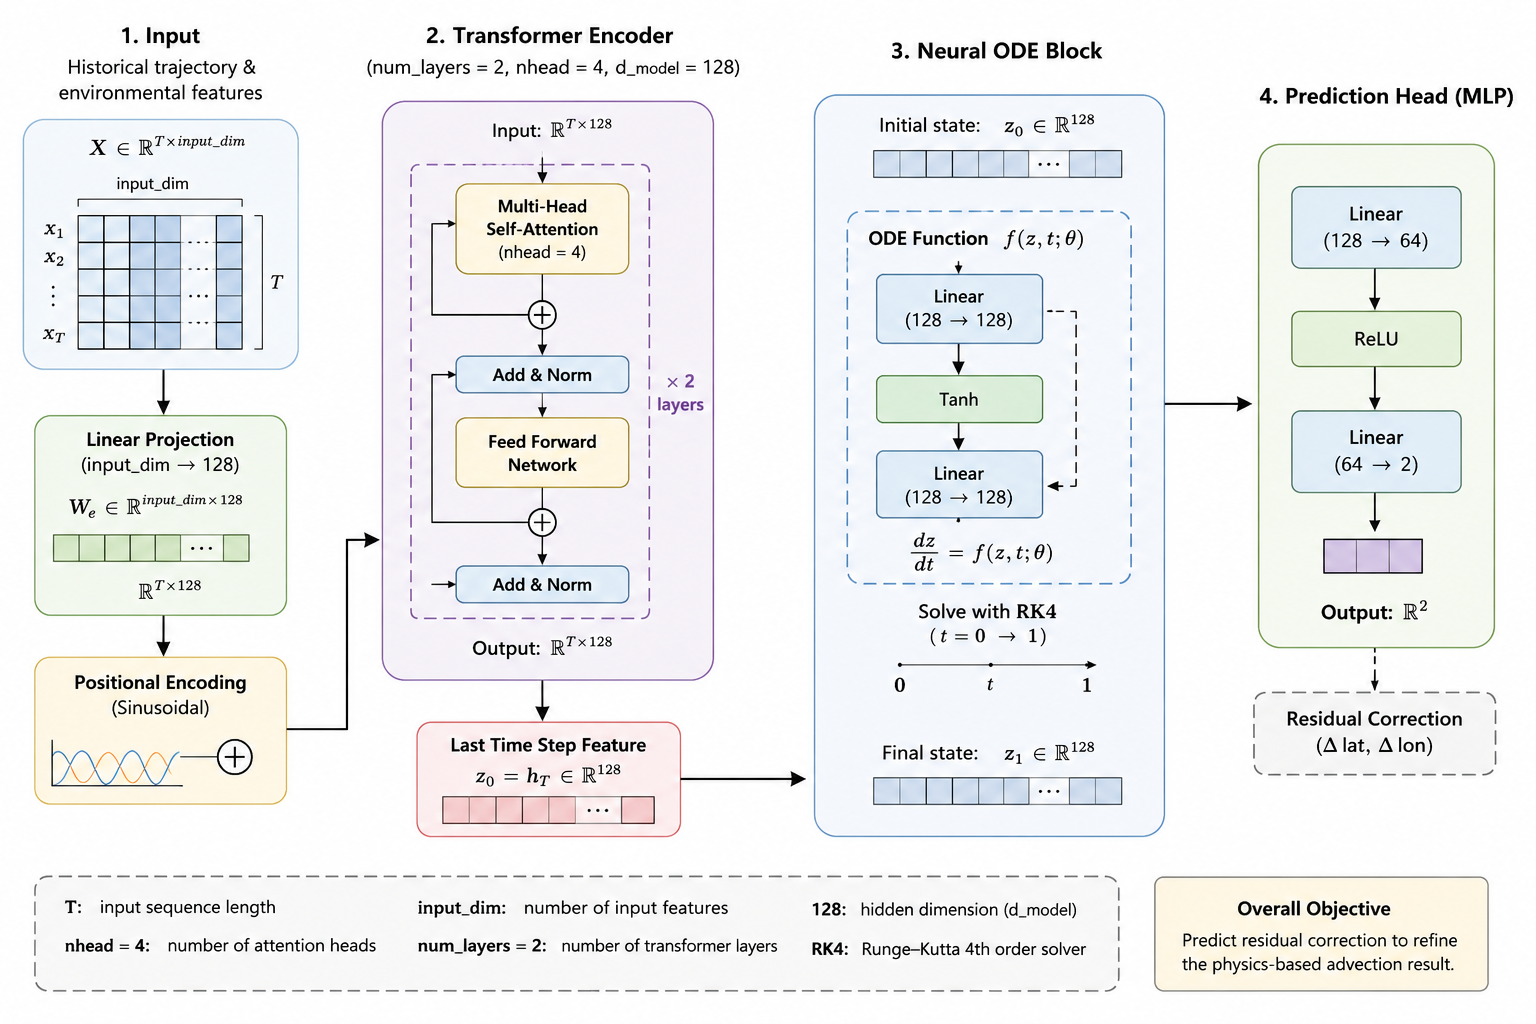
\includegraphics[width=0.8\linewidth]{transformer.png}
    \caption{Model Architecture}
    \label{fig:placeholder}
\end{figure}

\section{Loss Function}

\subsection{Prediction Loss}

The training objective primarily minimizes residual prediction error:

\begin{equation}
\mathcal{L}_{MSE}
=
\frac{1}{N}
\sum_{i=1}^N
||
\hat{r}_i - r_i
||^2
\end{equation}

The implementation additionally uses Smooth L1 loss during validation for robustness.

\subsection{Physics Regularization}

To stabilize residual magnitude, an auxiliary physics regularization term is added:

\begin{equation}
\mathcal{L}_{phys}
=
\frac{1}{N}
\sum_{i=1}^N
||\hat{r}_i||^2
\end{equation}

The final objective becomes:

\begin{equation}
\mathcal{L}
=
\mathcal{L}_{MSE}
+
\lambda
\mathcal{L}_{phys}
\end{equation}

where:$\lambda = 0.01$ controls the regularization strength.

\section{Training Strategy}

\subsection{Optimization}

    The framework uses AdamW optimization: learning rate: $10^{-4}$, weight decay: $10^{-5}$.AdamW improves generalization by decoupling weight decay from adaptive optimization.

\subsection{Learning Rate Scheduling}

A ReduceLROnPlateau scheduler is used: factor: $0.5$, patience: $3$ epochs.This strategy reduces learning rate when validation performance stagnates.

\section{Evaluation Metrics}

\subsection{RMSE in Geographic Space}

Latitude RMSE:

\begin{equation}
RMSE_{lat}
=
\sqrt{
\frac{1}{N}
\sum_i
(\hat{y}_{lat,i}-y_{lat,i})^2
}
\end{equation}

Longitude RMSE:

\begin{equation}
RMSE_{lon}
=
\sqrt{
\frac{1}{N}
\sum_i
(\hat{y}_{lon,i}-y_{lon,i})^2
}
\end{equation}

\subsection{Geodesic Error}

To measure real-world trajectory accuracy, Haversine distance is used.

For two geographic coordinates:

\begin{equation}
(\phi_1,\lambda_1)
,
(\phi_2,\lambda_2)
\end{equation}

The geodesic distance is:

\begin{equation}
d
=
2R
\arcsin
\left(
\sqrt{a}
\right)
\end{equation}

where:

\begin{equation}
a
=
\sin^2\left(\frac{\Delta \phi}{2}\right)
+
\cos(\phi_1)
\cos(\phi_2)
\sin^2\left(\frac{\Delta \lambda}{2}\right)
\end{equation}

and $R=6371$ km is Earth's radius.

The following statistics are computed:

\begin{itemize}
    \item mean geodesic error,
    \item median geodesic error,
    \item P90 geodesic error.
\end{itemize}

\section{Experimental Results and Analysis}

Example evaluation results:

\begin{table}[H]
\centering
\begin{tabular}{cc}
\toprule
Metric & Value \\
\midrule
Latitude RMSE & 0.0591 \\
Longitude RMSE & 0.7425 \\
Mean Geodesic Error & 8.57 km \\
Median Geodesic Error & 5.23 km \\
P90 Geodesic Error & 14.96 km \\
\bottomrule
\end{tabular}
\caption{Prediction Performance of the Proposed Model}
\end{table}

\subsection{Performance Interpretation}

The results demonstrate several important characteristics:

\begin{enumerate}
    \item The physics-advection baseline significantly stabilizes prediction.

    \item Residual learning reduces the burden on the neural network.

    \item Transformer attention effectively captures temporal dependencies.

    \item Neural ODE improves latent trajectory smoothness.

    \item Median geodesic error is substantially lower than mean error, indicating that large-error outliers are relatively infrequent.
\end{enumerate}

\subsection{Longitude Error Analysis}

Longitude RMSE is larger than latitude RMSE. Possible reasons include:

\begin{itemize}
    \item east-west ocean current variability,
    \item coordinate scaling sensitivity,
    \item accumulated advection uncertainty,
    \item unresolved mesoscale eddies.
\end{itemize}

The longitude conversion factor:

\begin{equation}
\cos(\phi)
\end{equation}

may also amplify instability at high latitude regions.

\subsection{Training Dynamics Analysis}
\begin{figure}
    \centering
    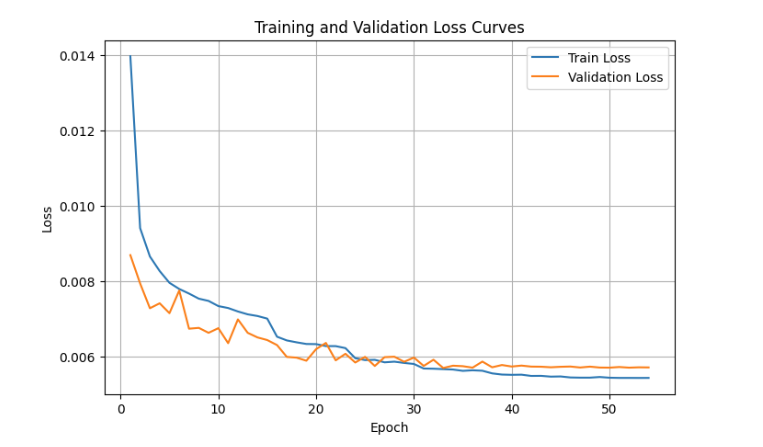
\includegraphics[width=0.5\linewidth]{loss_1.png}
    \caption{Caption}
    \label{fig:loss}
\end{figure}
Figure \ref{fig:loss} presents the training and validation loss curves of the proposed Transformer-ODE model. Both losses decrease rapidly during the first few epochs and gradually converge after approximately 30 epochs, indicating stable optimization and successful convergence. Furthermore, the training and validation losses remain close throughout training, suggesting that the model does not suffer from severe overfitting.

However, despite the stable convergence behavior, the Transformer-based model achieves inferior prediction accuracy compared with the LSTM baseline. Several factors may explain this phenomenon.

First, the trajectory sequences used in this study are relatively short and exhibit strong temporal continuity. Under such conditions, the recurrent inductive bias of LSTM is particularly effective because information is propagated sequentially through hidden states, naturally capturing local temporal dependencies. In contrast, the self-attention mechanism in Transformers is primarily designed to model long-range interactions and may not provide significant advantages when the sequence length is limited.

Second, the available training dataset is relatively small compared with the data scale typically required by Transformer architectures. While LSTM contains fewer parameters and imposes stronger structural priors on sequential data, Transformers generally rely on larger datasets to learn meaningful attention patterns. Consequently, the Transformer encoder may not fully exploit its representation capacity in this application.

Finally, ocean drifter trajectories are largely governed by continuous physical processes, resulting in smooth and slowly varying motion patterns. Such dynamics are often well aligned with the memory-cell structure of LSTM, whereas the global attention mechanism may allocate modeling capacity to less informative temporal interactions, reducing prediction efficiency.



\end{document}
```
